%!TEX root = ../thesis.tex
%*******************************************************************************
%****************************** Fourth Chapter *********************************
%*******************************************************************************

\chapter{Design of a bioelectrical impedance plethysmography device}
\label{chapter design}

\ifpdf
    \graphicspath{{Chapter4/Figs/Raster/}{Chapter4/Figs/PDF/}{Chapter4/Figs/}}
\else
    \graphicspath{{Chapter4/Figs/Vector/}{Chapter4/Figs/}}
\fi


As mentioned before, there are multiple applications where impedance plethysmography can be applied. Thus far though, this has only been achieved by devices that can only provide either basal impedance (DC), waveform (AC) or single channel application. This work is aimed to design a device that can be used to encompass any of the previous applications using a single apparatus. This device should be able to accommodate the characteristics described in a multi-channel device.  

Designing an impedance device necessitates functional knowledge about the electrical characteristics of the load under test. Nonetheless, meeting patient safety is a good starting point for the recommendations. This implies that the amount of current to be driven by the device should be imperceptible within the limits of the safety standards. To that end, one of the first recommendations is to be able to operate by batteries as a class B device in order to ensure that electrical currents are floating in the patient and guarantee that current will flow through the segment to be studied. The level of current sensation is predicated on factors including gender and is also predicated on the electrode geometry. However, Brown et al.~\cite{brown1998medical} have established a threshold current that is frequency dependent where \SI{5}{\mA} signifies the limit for sensory nerve stimulation and shock sensation. The device designed can deliver as many as four levels of current using a dip-switch (\SIlist{1;2;3;4}{\mA}). For the purpose of this document, the current was fixed at \SI{4}{\mA} which provided excellent sensitivity for the system. 

With regard to the electrical current delivered by the device, a programmable wave generator with a potential of delivering up to \SI{10}{\MHz} sinusoidal waveforms was incorporated into the design. However, as per the literature that gauges impedance, plethysmography can be achieved with frequencies between \SIrange[scientific-notation = engineering]{20}{200000}{\hertz}. Therefore, a sinusoidal wave of \SI{50}{\kilo\hertz} was used during the experimental procedure.

\section{Electrodes topology and location}
\label{section design electrodes}
As described in the section \ref{section iPG electrodes}, bioelectrical impedance plethysmography measurements can be attained with two electrodes topologies: bipolar and tetrapolar. Bipolar lacks two electrodes points to measure impedance. When taking the measurements with bipolar electrodes, a problem arises in that the impedance of the electrodes might be greater than the biological tissue itself, which can significantly affect the measurement. In the majority of the cases, it is quite difficult to differentiate the electrode impedance from tissue one \cite{brown2000bipolar}. Tetrapolar configuration requires four contact points; a pair of electrodes injects current, whereas another couple sense the voltage. Using tetrapolar arrangement minimises the decline in voltage during the measurements because the impedance of potential sensing amplifier is bigger than the interface electrode-skin. This means that electrical current would not flow between the electrodes and voltage amplifier. For this reason, a measurement of four electrodes was decided as the optimal method while designing the instrument. 

Positioning the electrodes close to the main vessel improves the response of this system since there is more conductive material where the electrical current can flow through. Figure~\ref{fig:electrode} illustrates the position of the electrodes to take measurements from the device. According to the arm anatomy, the radial artery is an ideal site to use one of the current electrodes. The other one was placed close to the brachial artery around the cubital fossa region where this vessel is in closer proximity to the surface. The sensing electrodes were placed towards the right hand side on the elbow, which is the nearest point to the brachial artery connected to the radial artery thus forming the ideal loop to detect the changes in impedance $\Delta Z$.  

\section{Bioelectrical impedance device modules}
A modular approach was used when designing the bioelectrical impedance device. Using this technique helps in isolating errors without manufacturing an entirely new system. It also allows the experimentation of different circuits to get the most suitable solution in order to obtain the most acceptable waveforms. During its development, different methods were tested to drive current, generate waveform or measure impedance. Towards the end, this solution was seen to present the best results. The optional modules will not be included in this thesis since they were excluded from the studies presented here.

Figure \ref{fig:electrode} illustrates the block diagram of the instrument. Operating the device requires four ECG electrodes: a battery bank, a DAQ card and a PC with LabView \cite{LabView:2016} installed. In general, some of the characteristics of this instrument are: differential sine wave generation through a DDS controlled by an Arduino MCU whose operation range varies from \SI{10}{\Hz} to \SI{25}{\MHz}. However, the frequency of operation of this device has been locked to \SI{50}{\kHz} \rvmynote{Check a paper for the frequency of operation}. Four different levels of differential current can be supplied \SIlist{1.33;2.16;3.60;4.36}{\mA}. The system senses the current delivered by electrode $E_4$ along with the potential forearm between electrodes $E_2$ and $E_3$; accordingly, the gain can be modified using dip-switches. The value peak of the measured current and potential is extracted via an envelope detector using \textit{"super diodes"}. A selection of filters cleans-up the signal and extracts the arterial pulses.

\begin{figure}[!htpb]
	\centering
	\includegraphics[width=12cm,keepaspectratio]{figure1}	
	\caption[General concept of the designed bioelectrical impedance device]{General concept of the designed bioelectrical impedance device. It also includes the position of the electrodes in the forearm.}
	\label{fig:electrode}
\end{figure}

The proposed system can be subdivided into two sections: 1) front-end, which is the part of the device that interacts directly with the limb under test; and 2) back-end, which performs the wave generation, signal conditioning, computational calculation, and data representation. The figure \ref{fig:block} displays the general schematic of this proposed device. The features and characteristics of each module will be illustrated as follows. The full schematics and part of the code used to control the DDS can be found in the Appendix section.


\begin{landscape}\centering
	\vspace*{\fill}
	\begin{figure}[!htp]
		\includegraphics[height=0.59\textheight,keepaspectratio]{figure2}
		\caption{Block diagram of impedance plethysmography device}
		\label{fig:block}
	\end{figure}
	\vspace*{\fill}
\end{landscape}

\subsection{Power supply module}
\label{section design battery}
Implementing an effective design requires good power supplies that can provide steady voltage output and sufficient current required by the circuitry. Due to the need for applying floating currents, a power supply was designed to operate using batteries by minimising ground loops and increasing patient safety.  The selection of this method of supplying power lessens the likelihood of electric shocks and attaining dangerous voltage levels. For these reasons, a couple of batteries A512/2 S (Sonnenschein) were used to power all the circuits. These cells provide \SI{2}{\ampere\hour} of capacity per bank.

Some of the unique features needed for power supply includes the ability to provide a dual voltage (\SI{\pm 12}{\volt}) because some Op-Amps require this level of supply to achieve maximum gain and low energy supply (\SI{5}{\volt}) which is essential for some digital components. The positive and negative voltages can be obtained by using one cell bank with normal polarisation and keeping the other one inverted. 

In summary, the following table illustrates the characteristics and IC's used in the power supply module. This includes level voltages, output current per channel and the specific function of each voltage level. 

\begin{table}[!htpb]
	\caption{Components of the Power Supply and its functions}
	\centering
	\label{table:power supply details}
	\begin{tabular}{p{2 cm} p{2 cm} c p{6 cm}}
		\toprule
		\centering{\textbf{Voltage supply}} & \centering{\textbf{Current supply}} & \centering{\textbf{IC}} & \centering{\textbf{Function}} \tabularnewline \midrule
		+\SI{12}{\volt} & \SI{1.5}{\ampere} & LM317 & Power supply for single and dual Op-Amps, In-Amps and as power supply for +\SI{5}{\volt} \tabularnewline \midrule 
		-\SI{12}{\volt} & \SI{1.5}{\ampere} & LM337 & Negative power supply for single and dual Op-Amps and In-Amps \tabularnewline \midrule 
		\SI{5}{\volt} & \SI{100}{\milli\ampere} & AP117E50G & Power supply for digital components working at TTL level \tabularnewline \bottomrule 
	\end{tabular}
\end{table}

The schematic circuits for the power supply designed are mentioned in the appendix \ref{Appendix: Power Supply}, figure \ref{Appendix: Power Supply}. Operating the iPG device requires positive (VIN+) and negative (VIN-) supplies that can be provided by any external power. For safety purposes, batteries were the source of choice. The table \ref{table:power supply details} shows the components employed in the implementation, which operates within the desired appropriate range as required by the device. The regulators LM3XX are voltage variable regulators. However, their output was set to \SI{\pm 12}{\volt} for each source using the appropriate selection of resistors. The capacitors which were added to all the regulators were selected in accordance to the manufacturer's recommendation to evade the prospects of any ripple at the output voltage.

In Altium Designer a PCB of \SI{50}{\milli\meter} x \SI{50}{\milli\meter} was produced considering input and ports in addition to indicators and sensors. For instance, the ports included three input voltage pins VIN+, VIN- and ground (GND) coming from the batteries, along with an eight-pin male connector that provides regulated board to the next board. These indicators and sensors included a dip-switch working as power ON/OFF button, a set of three red-LED indicating the power of +\SI{12}{\volt}, -\SI{12}{\volt} and \SI{5}{\volt}, and a three-pin port connected to the ADC port of the microcontroller which monitors the batteries' capacity. It also includes additional regulated voltage ports in order to feed other external modules.

\subsection{Direct digital synthesis (DDS) module}
\label{section DDS}
Following the block diagram from left to right illustrated in the figure \ref{fig:block}, the first part shows the wave generator. This section of the circuit produces the sinusoidal wave required to take the impedance measurements. This waveform needs to be low in distortion and noise. This signal was created using a programmable direct digital synthesis (DDS) integrated circuit (IC) that can produce sine waves from \SI{10}{\hertz} to \SI{25}{\mega\hertz}. The IC used here is the AD5930 (Analogue devices). In summation, a DDS creates a wave in accordance to a table of digital words in memory fed to a DAC that then produces the analogue equivalent. This IC requires a set of instruction to be able to operate. 

In the appendix \ref{Appendix: DDS PS}, the figure \ref{fig:DDS PS} shows the schematic used in the design of the wave generator. Owing to the noise that a digital circuit would feed into an analogue system, a separate power supply powers up this module. For this purpose, two voltage regulators (AP117E50G) provide \SI{5}{\volt} energy sources for digital and analogue components using two separated ground paths (GND - AGND). In addition, a \SI{3}{\volt} reference is needed for the oscillator to operate - which is supplied by the IC REF196. The DDS requires an external clock in order to work. Therefore, a \SI{50}{\mega\hertz} oscillator provides the desired clock signal.

A microcontroller ATMEL (Arduino) controls the DDS sending commands via serial peripheral interface bus (SPI) transmission interface. By making use of an instruction set by the manufacturer, it is possible to set the oscillation frequency of the sine wave and start/stop the signal generation. The appendix \ref{Appendix: Arduino} shows the code used to communicate with the PC and send commands to the DDS. The waveform generated by the DDS is differential, implying that there are two sine waves outputs in a counter-phase (\SIlist{0;180}{\degree}). The DDS provides a current output of \SI{3}{\mA} which is transformed to an electrical voltage using a \SI{200}{\ohm} resistor at the output of the IC, setting the output at approximately \SI{600}{\mV}. A set of capacitors also filters high-frequency noises. The connection between the microcontroller and other boards is made possible using ribbon cables. 

\subsection{Differential amplifier gain module}
The following stage consists of a differential voltage amplifier which, as its name suggests, amplifies the sinusoidal waveform coming from the DDS. The gain of this amplifier can be modified using a set of resistors at each side of the amplifier. It can also be adjusted to 16 different combinations of gain using resistors of \SIlist{1;2;3;4.99}{\kohm}. Moreover, the gain can be adjusted from \si{0.49} to \si{4.99}. As a result, the DDS' output voltage changes in accordance to the gain determined in the differential amplifier. 

The IC AD8137 was the main component of the DGA \cite{ad:AD8137}. Low tolerance resistors were placed at each channel to achieve a steady gain at the output. Since the DGA needed a separate power supply to operate within the limits of the batteries, a dual power supply of \SI{6}{\volt} and -\SI{6}{\volt} was designed using the IC LF60CDT and LM337 \rvmynote(Add data-sheet of these elements), respectively. Since the latter is a variable voltage regulator, a set of resistors was used to adjust the level of regulation to the desired level. The schematic circuits can be found in the appendix \ref{Appendix: DGA}, figures \ref{fig:DGA PS 6} and \ref{fig:DGA PS -6}

Owing to the fact that the DDS provides a DC coupled sine waveform and high-frequency noises, the input of the DGA incorporates a band-pass filter, formed by a DC blocking capacitor along with a low pass filter set to \SI{1}{\mega\hertz}. The output of this differential amplifier also includes another set of passive band-pass filters to eliminate any residual noise. The figure \ref{fig:DGA} in the appendix \ref{Appendix: DGA} shows the schematic. 

\subsection{Modified Howland Amplifier module}
\label{section MHC}
This is a very popular circuit method used in bioimpedance analysis (BIA) measurements \cite{aroom2009bioimpedance}, tissue characterization \cite{bertemes2002tissue,ross2003current}, electrical impedance tomography (EIT) and diagnosis of breast cancer \cite{zou2003review,saulnier2007electrical}. It can be constructed using a single operational amplifier (Op-Amp) as well as a handful of resistors \cite{sheingold1964impedance}. The Figure \ref{fig:mhc} illustrates the MHC configuration that offers wide bandwidth operation and low power consumption. 

Subsequently, a transconductance amplifier is used to convert the voltage coming out from the differential amplifier into an electrical current. Selected current will be passing through the patient. The chosen configuration is a modified Howland circuit set to \SI{1}{\milli\siemens} of gain.

The Op-Amp selected for this design was the AD8066 (Analog Devices), a dual Op-Amp that offers high bandwidth of \SI{145}{\mega\hertz}, high input impedance of \SI{1000}{\giga\ohm} @ \SI{4.5}{\pF}, low noise of \SI{7}{\nano\volt\per\sqrt{Hz}} at \SI{10}{\kilo\hertz}, open loop gain of \SI{113}{\decibel} and CMMR of -\SI{100}{\decibel}~\cite{ad:AD8066}. All these characteristics made this Op-Amp an ideal choice to implement a MHC.

\begin{figure}[!htpb]
	\centering
	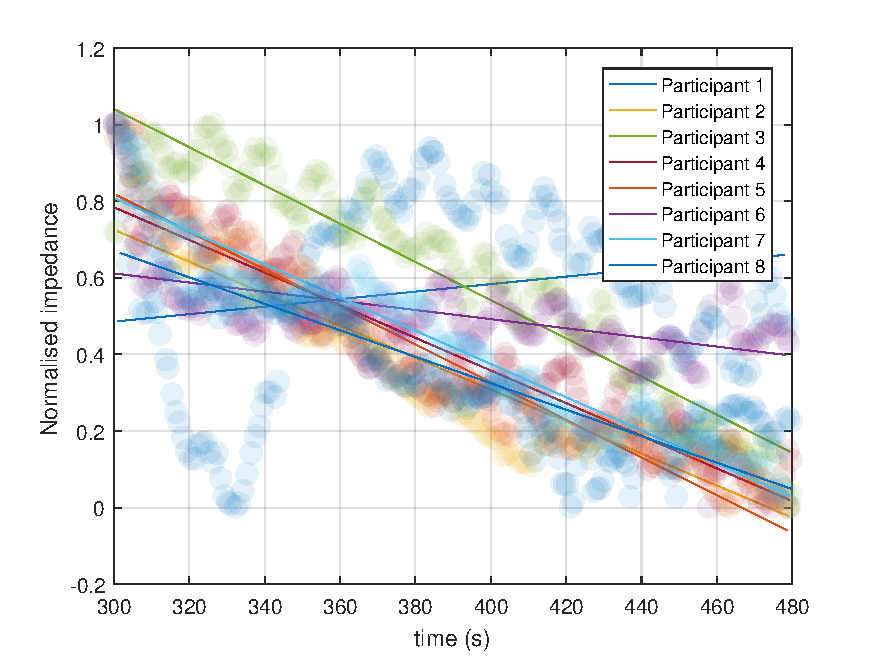
\includegraphics[width=9cm,keepaspectratio]{figure3}  
	\caption{Modified Howland circuit schematic}
	\label{fig:mhc}
\end{figure}

The MHC design requires low tolerance resistors to minimise potential errors caused to the system. As a result, the resistors of \SIlist{1;100}{\kohm} with a tolerance of \SI{0.1}{\percent} were used in the final implementation. Figure \ref{fig:mhc} shows the implemented schematic of the differential MHC, only the top Op-Amp is analysed to prove that the equivalence was met, the one on the bottom follows the same equations but with an inverted output. The circuit's resistors from the equation are equivalent to the followings: $R_{2A}=R_1, R_{2B}=R_2, R_1 = R_3 + R_4, R_3 = R_5$ and $R_4 = R_6$. Thus, the equation can be re-written as follows: 

\begin{align}
	\label{eq:Req}
	\frac{R_1 + R_2}{R_3 + R_4} = \frac{R_6}{R_5}
\end{align}

where $R_1=R_4=R_5=R_6=100K\Omega$ and $R_2=R_3=1K\Omega$. Finally, the resistor equivalence is calculated as shown by equation \ref{eq:Req}. 

The transconductance of this circuit was calculated from equations \ref{eq:Req}. After the same resistors equivalence that were previously described, the positive transconductance $(G^+_m)$ and negative transconductance $(G^-_m)$ were calculated as described by the following arithmetical operations:

\begin{align}
	\label{eq:G+}
	G^+_m=\frac{i_{out}}{v_{in+}}=\frac{100K\Omega + 1K\Omega}{101K\Omega \times 1K\Omega}=\frac{101K\Omega}{101M\Omega}=1\times10^{-3}S 
\end{align}

\begin{align}
	\label{eq:G-}
	G^-_m=-\frac{i_{out}}{v_{in-}}=\frac{100K\Omega + 1K\Omega}{101K\Omega \times 1K\Omega}=\frac{101K\Omega}{101M\Omega}=-1\times10^{-3}S 
\end{align}

As can be seen from \ref{eq:G+} and \ref{eq:G-}, the transconductance in both feedbacks is equivalent to \SI{1}{\milli\siemens}. The negative sign in $G^{-}_m$ is caused by a phase shift of \SI{180}{\degree}. Due to the fact that top and bottom Op-Amps shown in figure \ref{fig:mhc} has the same design, the total transconductance of the circuit in differential mode is equal to \SI{1}{\milli\siemens}. In other words, for every volt generated at the input (pins input- and input+) the output produces \SI{1}{\mA} of electric current. By interfacing the previous DGA module with this one, it becomes possible to produce sixteen different levels of current. Nonetheless, for the purpose of setting the instrument, only one switch should be activated at a time to provide fixed currents of \SIlist{1.33;2.16;3.60;4.36}{\mA}.

The design also includes a high-pass filter at the output of the circuit. These RC networks act as DC decoupling and ground clamping because floating loads can witness DC offset coming from the signal, which might cause an error in the current. However, these capacitors also have an effect on the bandwidth of the circuit. The resistor, which could be the potential output impedance of the MHC, was chosen to be as high as possible (\SI{1}{\mega\ohm}).

\begin{align}
	\label{eq:MHC filter}
	f_c = \frac{1}{2 \pi R C} = \frac{1}{2 \pi \SI{1}{\mega\ohm} \SI{1}{\micro\farad}} = \SI{0.159}{\hertz}
\end{align}

The design also included a dual power supply of \SI{5}{\volt} and -\SI{5}{\volt} provided by the IC's AP117E50G and L79L05, respectively. The final circuit schematics, which include the MHC and power supplies, are shown in figures \ref{fig:MHC}, \ref{fig:MHC PS 5} and \ref{fig:MHC PS -5}. From that design, the PCB was produced using the same manufacturing method of the previous ones/

\subsection{Current and voltage sensing module}
\label{section V&I sense}
As shown in figure \ref{fig:mhc}, at the output of the transconductance, amplifier resistors $R_s$ of \SI{10}{\ohm} were placed at each side of the differential output. These small resistors sense the electrical current passing through the unknown load. Using Ohm's law $v=R \times i$ it is possible to convert this current into a proportional voltage value. However, by combining a small flowing current around $mA$ with a tiny resistor value, the voltage obtained is in the order of $mV$. Consequently, this resultant voltage is too close to the noise level, and hence cannot be detected by any analogue to digital converter. Therefore, using a high input impedance amplifier is important to avoid current leakage through the current sensing IC and improve the signal to noise ratio.  

The most suitable device for this design was the In-Amp AD8421~\cite{ad:AD8421}. Some of this device's features include the low noise of \SI{3.2}{\nano\volt\per\sqrt{Hz}} at \SI{1}{\kHz}, a high bandwidth \SI{10}{\MHz} at a unitary gain, a high CMRR of \SI{80}{\decibel} at \SI{20}{\kHz} and dual supply operation within the range of the power supply designed. This component also benefits from adjustable gain using external resistors between pin 2 and 3. In fact, a four dip-switch with four different resistor values was included in the design process to increase the gain of the voltage detected as shown here \ref{fig:peak}. Hence, if the device uses a small value of current (\SI{1.3}{\mA}), it becomes possible to adjust the gain derived at this stage to obtain a more accurate reading.

\begin{figure}[!htpb]
	\centering
	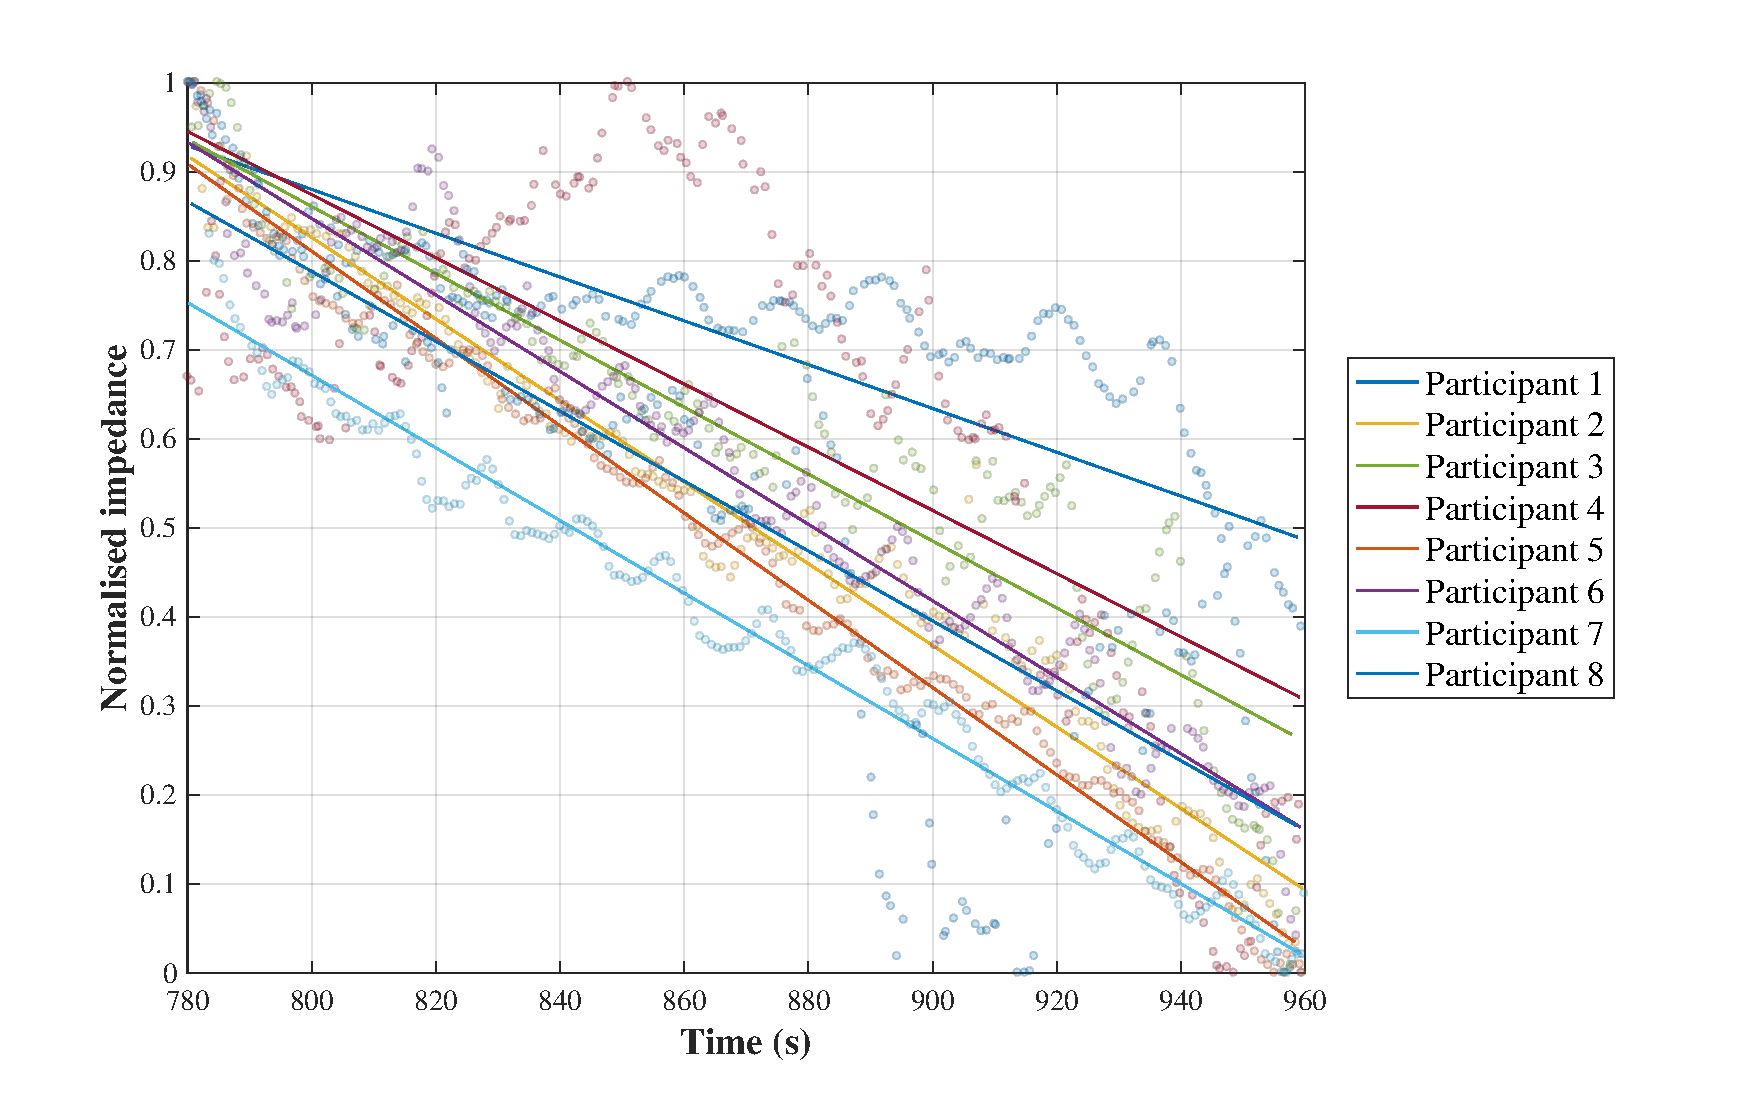
\includegraphics[width=8cm,keepaspectratio]{figure4}
	\caption{Current sensing circuit schematic}
	\label{fig:peak}
\end{figure}

Likewise, this same circuit was used to detect the voltage produced by the limb segment. When the biological sample is excited with an electrical current, it leads to the emergence of a potential, as described in section \ref{section impedance principle}. To that end, the electrodes $E_2$ and $E_3$ (see figure \ref{fig:electrode}) provided the connection towards the input pins of the In-Amp AD8421 \cite{ad:AD8421}. The robust input impedance of this IC and typical input bias current of \SI{1}{\nA} guarantees minimal voltage drop from the interface electrode-skin. Therefore, the maximum error introduced by this voltage drop is close to \SI{0.0001}{\percent} per mA which flows through the body segment. The gain of the IC can be modified using its gain pins, increasing the dynamic range of the sensing circuit. Consequently, a dip-switch 4 SPST was used to provide as many as 16 different combinations of amplification that could be adapted as per the nature of the signal. The final schematic can be appreciated in the appendix \ref{Appendix: VSense} figure \ref{fig:Voltage sense}.

A sensing module was manufactured by combining the current sense and two channels of potential. Channel one was used to detect the voltage produced by the limb segment, whereas the second channel will be used for future studies carried out on differential impedance measurements. The only difference between the current and potential circuits is the selection of gain resistors that were allocated in accordance to the range of the signals to be detected. The output signal produced by this module is then passed through a peak and envelope detection circuit as described in the next section. 

\subsection{Envelope detection and AC extraction circuit module}
\label{section material envelope}
This module has two functions: the first one detects the peak value of the current and voltage sensing circuit, whereas the other one extracts the plethysmography waveform contained within the baseline impedance. Hence, three output signals are produced by this module. The first signal is a DC voltage equivalent to the amplitude of the voltage detected by the current sense path denominated $I_{DC}$. The second output channel is a DC signal equal to the potential detected on the limb segment denoted by $Z_{DC}$. The third one is an AC signal that represents the dynamic plethysmography signal or arterial pulse amplitude called $Z_{AC}$

The envelope or peak detection is achieved using the combination of an active diode configuration and a hold circuit. The first part of this circuit was created using an Op-Amp TL08XX \cite{ti:TL08xx} as well as a diode 1N4148. The combination creates a ''super diode'' or ''perfect diode'' circuit. Thus, the Op-Amp complements the diode's voltage drop when the signal crosses zero. The negative feedback resulting from the output of the diode towards the negative pin of the Op-Amp mitigates the diode's voltage drop. Resultantly, the output signal at the cathode's diode is essentially a half-wave rectified waveform crossing by zero. The figure \ref{fig:envelope} shows a model of this circuit. 

\begin{figure}[!htpb]
	\centering
	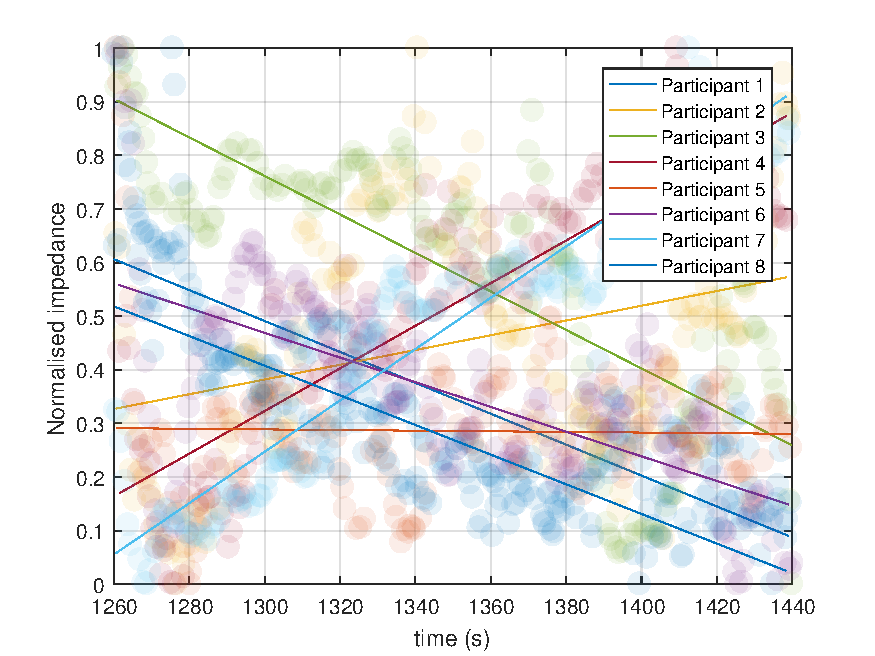
\includegraphics[width=7.3cm,keepaspectratio]{figure5}
	\caption{Envelope detection circuit schematic}
	\label{fig:envelope}
\end{figure}

The signal obtained by the super diode circuit is passed on to a hold circuit denoted by $C_E$ and $R_E$ in the figure \ref{fig:envelope}. This RC configuration keeps its charge for a period of the signal produced by the wave generator, as described in section \ref{section DDS}. The frequency for measuring impedance plethysmography was selected at \SI{50}{\kHz} which implies that the distance peak-to-peak is \SI{20}{\micro\sec}. The time constant ($\tau$) of the RC network can be calculated by the following equation:

\begin{align}
	\tau = RC = 1 \mu F \times 120K\Omega = 0.12 Sec
\end{align}

The holding time of the RC network at $5\times\tau$ is \SI{0.6}{\sec}, which implies that this RC combination can detect the peak of a signal with a frequency as low as \SI{1.66}{\Hz}. Consequently, this circuit produces a DC signal equivalent to the peak value of the input signal. This makes it possible to generate the signals of channels $I_{DC}$ and $Z_{DC}$ which are the voltage representations of the current driven by this device and the voltage provided by the unknown load. Therefore, these two signals make it possible to quantify the basal impedance by dividing the potential over the current values. The calculation of impedance is performed during the post-processing stage in Matlab \cite{MATLAB:2016}. Consequently, these signals must be digitised using DAC cards. Hence, the output channels should provide a low impedance interface, which is achieved by passing these waveforms through buffers. The schematic implemented within the final circuit can be seen in the appendix \ref{Appendix: Envelope}, figures \ref{fig:envelope detector current} and \ref{fig:envelope detector voltage}.

By isolating and amplifying the dynamic component within the basal impedance, it is possible to extract the APA waveform. Therefore, the unbuffered signal from channel $Z_{DC}$ channel gets passed through a series of filters shown in figure \ref{fig:envelope detector voltage}. Following that schematic, a high pass filter (HPF) is used to remove the signal's DC components, which is possible by implementing a passive filter composed by capacitor and resistor $C_4$ and $R_5$, respectively. Notably, $R_5$ is virtually connected to ground (GND) through the negative pin of the Op-Amp. The cutting frequency of the HPF was calculated using the equation \ref{eg:fc1} - which demonstrates that this circuit section practically blocks any DC component of the impedance signal. 

\begin{align}
	\label{eg:fc1}
	f_c = \frac{1}{2 \pi R C} = \frac{1}{2 \pi 330K\Omega 4.7\mu f}=10.26 mHz
\end{align}

Subsequently, a second order active filter eliminates any high-frequency noise occurring within the plethysmography signal. The cut off frequencies were calculated as outlined in equations~\ref{eg:fc2} and~\ref{eg:fc3}. The first Op-Amp configuration is an inverting amplifier circuit with a frequency cut at \SI{10.61}{\Hz} and a gain in DC of \num{30.30}. The second Op-Amp configuration \SI{10.26}{\Hz} has an amplification factor in DC of \num{4.70}. 

In general, the extraction of the APA signal is achieved with a band-pass filter with low-frequency cut at \SI{10.26}{\milli\hertz} with a roll-off of \num{20} dB/decade as well as a high-frequency cut at \SI{10.26}{\Hz} with a roll-off of \num{40} dB/decade. Finally, the final output was passed on to a buffer configuring the channel $Z_{AC}$. The APA waveform is then amplified using a fixed gain of \num{142.41}.

\begin{align}
	\label{eg:fc2}
	f_c = \frac{1}{2 \pi R C} = \frac{1}{2 \pi 10M\Omega 1.5 nf}=10.61Hz
\end{align}

\begin{align}
	\label{eg:fc3}
	f_c = \frac{1}{2 \pi R C} = \frac{1}{2 \pi 47K\Omega 330nf}=10.26Hz
\end{align}

The envelope detection module was manufactured in accordance to these design considerations. The output channels from this PCB are the ports which are known as $I_{DC}$ or peak current value; $Z_{DC}$ or peak impedance potential and $Z_{AC}$ or arterial pulses.   

\section{Final assembly circuit}
\label{section design final}
The figure \ref{fig:assembly} shows the final circuit assembly. All these modules were fixed to a board, and the different circuit stages were interconnected using jumper cables. In the same board, a DAQ NI USB-6212 (National Instruments) was mounted to connect the output channels $I_{DC}$, $Z_{DC}$ and $Z_{AC}$. Additionally, in order to ensure a cohesive system, the Arduino MCU was also affixed and connected to the DDS module. 

As inputs and outputs, the instrument includes data and power ports. The data ports have two USB cables connected to the DAQ box and the Arduino PCB. They work as a digital data bus and system command controller, respectively. The system is powered by the battery bank using the PSU module. For this to happen, a 4-pins cable was designed as interface. The electrodes cables run from the MHC and sensing boards. These cables were designed using alligator clips that got hooked on to the electrodes end. 

\begin{figure}[!htpb]
	\centering
	\includegraphics[width=\textwidth,keepaspectratio]{figure_assembly}
	\caption{Representation in 3D of the modified Voltage sensing circuit module}
	\label{fig:assembly}
\end{figure}

\section{Conclusion}
\label{conclusion impedance device}
This section described the hardware design of an impedance plethysmography device which senses the current delivered as well as the potential generated by an unknown load in the forearm. The design of this device was replete with patient safety features by delivering an imperceptible electrical current. The electrical characteristics of the bioelectrical impedance device included a wave generator capable of producing a sine waveform of up to \SI{50}{\kHz} that was designed using a DDS with capabilities of frequency adjustment at the levels below \SI{100}{\kHz}. At this level of frequency, the current delivery needs to be less than \SI{5}{\mA}. The device was designed to operate over four different levels of current between \SIlist{1.33;2.16;3.60;4.36}{\mA} which was accomplished by implementing a Modified Howland Circuit. The measurement of impedance was made possible by measuring the delivered current and the potential measured. The sensing circuits were implemented using high input impedance instrumentation amplifiers to guarantee high noise rejection. 

One of the unique features of this instrument is the capability to produce not just the total impedance of a targeted segment of the limb, but also the arterial pulses amplitude. The two signals have been used separately to either measure volume changes using venous occlusion plethysmography \cite{mohapatra1979measurement, costeloe1980continuous, yamakoshi1980limb} or estimate blood flow beat by beat  \cite{porter1985measurement, corciova2011peripheral, brown1975impedance, marks1985computer}. However, the author was of the view that additional information should be obtained when combining both measurements. Therefore, it was imperative to design a device capable of providing both signals in real time, similar to the ones presented in the literature which primarily focused on one of the waveforms. 

Therefore, the impedance plethysmography device incorporated 5 output channels. The first channel named $I_{DC}$, provided the peak value of the electrical current being driven into the patient. Thus, it is possible to sense the impedance readings more accurately since the delivered current is constantly measured for real time measurements. The four other outputs are divided into two channels of potential measurement. Each of these channels sense the voltage when reading from the tissue. One of the channels labelled as $Z_{DC}$ provides readings of the peak voltage obtained from the patient. The other channel called $Z_{AC}$ displays the AC component of the impedimetric signal lying within the impedance measurements.  

There were some prerequisites to ensure the viability of this instrument being used at home. Ease of use was one of the first and biggest challenges to be addressed. The bioelectrical impedance device would have the potential of being used at home without the assistance of specialised personnel. The use of a tetrapolar electrode configuration increases the simplicity and usability of the device as compared to other devices that are used to measure changes of blood volume in the body. Using the same measurement point at all times ensures a more accurate reading. This means that having fixed accessible spots like elbows and wrists always a long way in taking a similar measurement. In future implementations, this issue could be addressed by using a sleeve that covers the limb and marks the position of electrodes points. 

Portability was another desired characteristic that may facilitate the use of this device at home. Using batteries to power the instrument may not only help in addressing this issue, but also in increasing patient safety. As mentioned in this chapter, the device was powered using two battery banks of \SI{\pm 12}{\volt} which allowed the device to be charged and transported. Being a battery-powered device, it can be used safely in patients. The instrument was driving floating loads, which implies that current cannot pass through the earth and cause potential harm to the patient. This issue was taken into consideration during the ethics approval and throughout the course of this experimental procedure which is described further in chapter \ref{chapter procedure}.




%********************************** %Nomenclature found  *************************************
\nomenclature[z-rc]{RC}{Resistor Capacitor}
\nomenclature[z-rc]{BIA}{Bioimpedance Analaysis}
\nomenclature[z-rc]{EIR}{Electrical impedance tomography}
\nomenclature[z-dds]{DDS}{Direct Digital Synthesis}
\nomenclature[z-dds]{DGA}{Differential Gain Amplifier}
\nomenclature[z-ic]{IC}{Integral Circuit}
\nomenclature[z-spi]{SPI}{Serial Peripheral Interface Bus}
\nomenclature[z-opamp]{Op-Amp}{Operational Amplifier}
\nomenclature[z-cmmr]{CMMR}{Common Mode Rejection}
\nomenclature[z-mhc]{MHC}{Modified Howland Circuit}
\nomenclature[z-inamp]{In-Amp}{Instrumentation Amplifier}
\nomenclature[z-adc]{ADC}{Analogue to digital converter}
\nomenclature[z-spst]{SPST}{Single Pole Single Throw}
\nomenclature[z-dc]{DC}{Direct Current} 
\nomenclature[z-ac]{AC}{Analogue Current}
\nomenclature[z-gnd]{GND}{Ground Point}
\nomenclature[z-pwv]{PWV}{Pulse Wave Velocity}
\nomenclature[z-hpf]{HPF}{High-Pass Filter}
\nomenclature[z-lpf]{LPF}{Low-Pass Filter}

